\documentclass[tikz,border=5pt]{standalone}
\usepackage{tikz}
\begin{document}
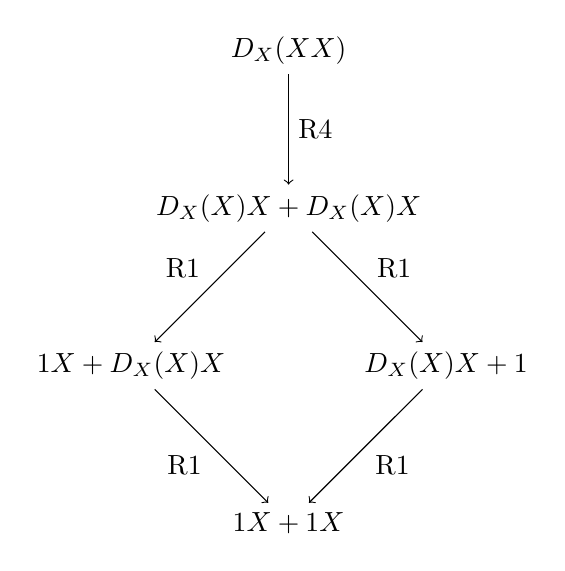
\begin{tikzpicture}

\node (a) at (0,0) {$D_X(XX)$};
\node (b) at (0,-2) {$D_X(X)X + D_X(X)X$};
\node (c) at (-2,-4) {$1X + D_X(X)X$};
\node (d) at (2,-4) {$D_X(X)X + 1$};
\node (e) at (0,-6) {$1X + 1X$};

\draw[->] (a) -- node[right] {R4} (b);
\draw[->] (b) -- node[above left] {R1} (c);
\draw[->] (b) -- node[above right] {R1} (d);
\draw[->] (c) -- node[below left] {R1} (e);
\draw[->] (d) -- node[below right] {R1} (e);

\end{tikzpicture}
\end{document}
